\capitulo{6}{Trabajos relacionados}
Además de este proyecto, ha habido otros similares en los que se trata de identificar el Parkinson mediante visión artificial con otro tipo de técnicas.

Dada la gravedad de la enfermedad, ha habido varios estudios aplicando diversas formas de detección de Parkinson para facilitar el trabajo de médicos, además de servir a modo de autodiagnóstico.

En este apartado se van a exponer aquellos trabajos que también se dedican a detectar el Parkinson y que están relacionados con este proyecto.

\subsection{A new computer vision-based approach to aid the diagnosis of Parkinson's disease}
Este trabajo~\cite{pereira2016new} consiste en detectar utilizando técnicas de visión artificial si una persona tiene Parkinson o no mediante dibujos de espirales realizados a mano por varias personas.

El primer paso es el de realizar una prueba en la que hay que dibujar las formas tal y como se aprecia en la figura \ref{fig:pruebapapel}, tan solo realizando los ejercicios c y d.

Posteriormente, estos ejercicios son digitalizados para realizar la extracción del dibujo realizado, los cuales se enumeran del 1 al 4 para el ejercicio c y del 5 al 8 para el ejercicio d. Dado que cada individuo realiza 8 dibujos, se acaban obteniendo unos datos. La recogida de datos se realizó tanto a pacientes diagnosticados como a control.

A continuación, el proceso se divide en dos pasos: procesado de imágenes y extracción de características.

El primer paso consiste en separar el dibujo de la persona (HT) del dibujo del papel (ET). Se utilizan técnicas de procesado como filtrado y morfología matemática.

\begin{figure}[ht]
	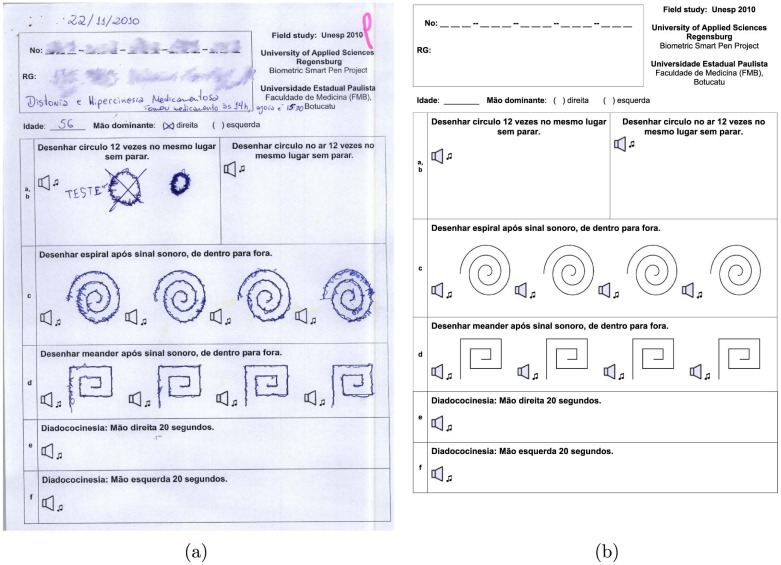
\includegraphics[width=1\textwidth]{prueba_papel}
	\caption{Prueba a papel que realizó una persona con Parkinson en este proyecto (a) y la hoja en blanco de la prueba (b)~\cite{pereira2016new}.}
	\label{fig:pruebapapel}
\end{figure}

A la hora de obtener el dibujo del paciente (HT), en primer lugar se filtran los dibujos para eliminar el ruido, y en el siguiente paso se utiliza una fórmula que actúe como umbral con el fin de obtener una máscara binaria \(M^{i}_{ET}\ (I)\), tal y como se muestra: 

\begin{equation}
	M^{i}_{ET}\ (I) = \left\lbrace\begin{array}{ll}
0~\text{if}~R^{i}~(I)<100\wedge G^{i}~(I)<100\wedge B^{i}~(I)<100 \\ 1~\text{otherwise,} \end{array}\right.
\end{equation}

\(R^{i}(I)\), \(G^{i}(I)\) y \(B^{i}(I)\) son los valores del espacio de color RGB del píxel \(i\). Una vez obtenida la máscara \(M^{i}_{ET}\ (I)\), se restan los píxeles de la imagen original, obteniendo únicamente el dibujo del paciente.

Por otro lado, se obtiene el dibujo de la prueba (ET) de una manera similar. Se utilizan filtrados para eliminar el ruido y, a continuación, se calcula un umbral mediante una fórmula para obtener una máscara \(M^{i}_{HT}\ (F)\) que en este caso no será binaria, ya que será necesario obtener el color del bolígrafo para poder separarlo y extraer el dibujo del fondo tal y como se muestra:
 
\begin{equation}
	M^{i}_{HT}\ (F) = \left\lbrace\begin{array}{ll}
		255\begin{split}&~\text{if}~|R^{i}~(F)-G^{i}~(F)|<40\wedge |R^{i}~(F)-B^{i}~(F)|<40~\wedge \\ & \wedge|G^{i}-B^{i}|<40 \end{split} \\ F^i~\text{otherwise,} \end{array}\right.
\end{equation}

\(F^{i}\) es la saturación de color del píxel \(i\). Al igual que sucedía en el proceso anterior, cuando se  obtiene la máscara \(M^{i}_{HT}\ (F)\), se restan los píxeles de la imagen original, obteniendo únicamente el dibujo de la prueba.

Finalmente, se obtienen dos imágenes en cada dibujo: el dibujo del paciente y el dibujo de la prueba, como se aprecia en la figura \ref{fig:resultado}.

\begin{figure}[ht]
	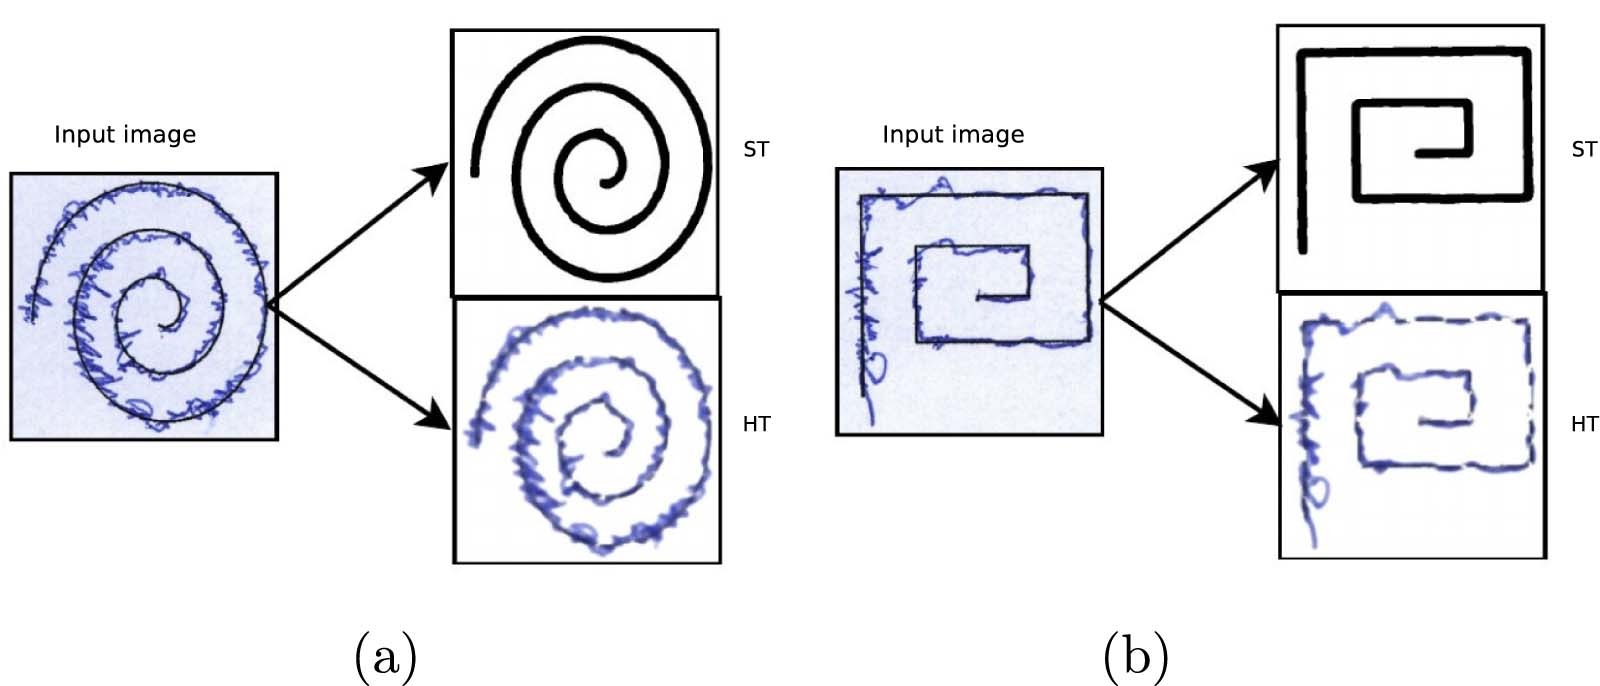
\includegraphics[width=1\textwidth]{resultado_dibujos}
	\caption{Resultado obtenido en cada dibujo del ejercicio c (a) y del ejercicio d (b)~\cite{pereira2016new}.}
	\label{fig:resultado}
\end{figure}

El segundo paso del proceso consiste en extraer características de los dibujos. Para ello se comparan las dos imágenes obtenidas en el primer paso para evaluar cómo de diferentes son. 

Para facilitar el proceso, se utiliza el algoritmo de adelgazamiento Zhang–Suen~\cite{zhang1984fast}, que resumidamente se encarga de hacer que las trazas de los dibujos aparezcan de forma más fina. Además, se corrigen algunas imperfecciones en las imágenes, como líneas discontinuas. Después, se enumeran algunos puntos en las imágenes y se compara la posición entre dos puntos equivalentes para conocer la desviación del dibujo del paciente con respecto al dibujo de la prueba, obteniendo varios datos con las características de los dibujos. También se obtienen datos obteniendo la distancia entre algunos puntos aleatorios de ambas espirales al centro, ya que la desviación del dibujo del paciente afecta también en su enfermedad de Parkinson. Finalmente, se entrenan los modelos para detectar el Parkinson con todos los datos obtenidos en el paso anterior.

El experimento que se llevó a cabo albergaba dos grupos de personas: uno con gente sin Parkinson y otro con gente con Parkinson. Además, se mezcló en ambos grupos los dos sexos y algún zurdo, frente a una mayoría diestra.

\subsection{Proposing a Three-Stage Model to Quantify
	Bradykinesia on a Symptom Severity Level
	Using Deep Learning}
Este proyecto~\cite{jaber2021proposing} es similar al que se trata en este TFG, ya que también se basa en recoger datos procesando la mano haciendo un movimiento de pinza.

Para ello, se procesan varios vídeos con la mano, tanto izquierda como derecha, habiendo además varios de control. El movimiento realizado debe ser lo más rápido y amplio posible durante 10 segundos.

El preprocesado se realiza utilizando VLC Player para obtener fotogramas de los vídeos. Con Python, y más concretamente, una biblioteca llamada LabelImg se anotan de forma gráfica objetos detectados en la imagen, como se puede observar en la figura \ref{fig:manoetiquetada}.

\begin{figure}[]
	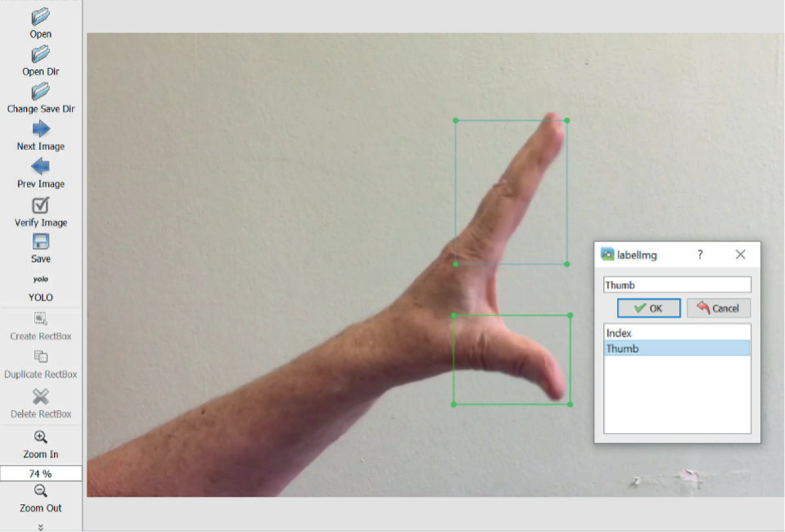
\includegraphics[width=1\textwidth]{mano_etiquetada}
	\caption{Mano con los dedos índice y pulgar etiquetados~\cite{jaber2021proposing}.}
	\label{fig:manoetiquetada}
\end{figure}

Eso servirá para recoger las coordenadas de los dedos índice y pulgar y anotarlos en un fichero de texto de la manera:
\begin{center}
	\texttt{< object - class >< x\_center >< y\_center >< width >< height >}
\end{center}

Utilizando la herramienta YOLO, se consigue que los vídeos sean procesados en tiempo real, y así, se obtiene más velocidad en el preprocesado.

Cada recuadro muestra el ID de la clase y la confianza de detección tal y como se ve en la figura \ref{fig:manoetiquetas}. El movimiento se conoce comparando las coordenadas del recuadro con las coordenadas del recuadro que tenía el fotograma anterior, lo cual se almacena para cada fotograma junto al momento en el que se calcula.

\begin{figure}[]
	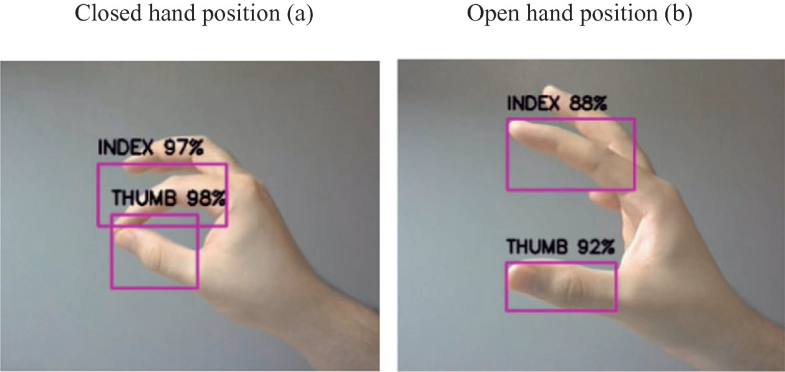
\includegraphics[width=1\textwidth]{mano_etiquetas}
	\caption{Detección realizada con un ajuste ideal~\cite{jaber2021proposing}.}
	\label{fig:manoetiquetas}
\end{figure}

En caso de haber ruido de fondo y/o una orientación de la mano diferente, podría afectar a la confianza de detección, empeorando los resultados obtenidos.

Estos datos obtenidos se utilizan para realizar cálculos con los que sacar conclusiones. Entre los cálculos se encuentran:

\begin{itemize}
	\item Separación: es el desplazamiento entre dos recuadros.
	\item Tiempo: se obtiene extrayendo el fotograma actual y restándole el anterior dividido entre los fotogramas capturados por segundo.
	\item Velocidad: se calcula con la diferencia de separación entre dos fotogramas contiguos dividido entre el tiempo.
	\item Ritmo: es el producto entre la diferencia de separación de dos fotogramas contiguos y su respectiva velocidad.
\end{itemize}

Finalmente, los datos se representan en gráficas observar las diferencias de las personas que padecen Parkinson de las que no y con ello alcanzar conclusiones.

\subsection{The discerning eye of computer vision: Can it measure Parkinson's finger tap bradykinesia?}
En este proyecto~\cite{williams2020discerning}, se ha querido conocer si es posible medir el Parkinson abriendo y cerrando los dedos en forma de pinza, de forma similar a como se hace en el trabajo que representa este documento.

Las mediciones están dentro de la escala MBRS (\textit{Modified Bradykinesia Rating Scale}), que evalúa la velocidad, la amplitud y el ritmo de los movimientos y de la escala MDS-UPDRS~\cite{goetz2008mds} (\textit{Movement Disorder Society revision of the Unified Parkinson's Disease Rating Scale}), que se encarga de evaluar aspectos que tiene el Parkinson con respecto a experiencias motoras y no motoras del día a día.

Como herramienta, se utilizó DeepLabCut, que es una herramienta muy similar a la biblioteca Mediapipe de Python que ya se ha explicado en este documento, en la que cualquier parte del cuerpo es marcada con unos puntos para obtener datos acerca de cómo se está moviendo. Sin embargo, para este proyecto sólo se utilizó la herramienta para las manos.

Los puntos de la mano, se utilizaron para conocer el movimiento de los dedos al realizar el movimiento de pinza, creando coordenadas de los dedos para cada vídeo. Estas coordenadas son las que se utilizaron para obtener la distancia entre los dedos. Además, al igual que en el proyecto que se presenta en el documento, en este también se utilizó el filtrado Savitzky-Golay para eliminar algunos errores que pudiera ocasionar la herramienta.

Los datos que se extrajeron sirvieron para obtener la amplitud, la velocidad y el ritmo del movimiento. Los datos se representaron en forma de gráfica, tal como se aprecia en la figura \ref{fig:grafica}. Para la amplitud se recogió la propia amplitud de la onda, para la velocidad se recogió el ratio medio de cambio de los puntos y para el ritmo se utilizó la transformación rápida de Fourier para encontrar la distribución de las frecuencias dentro de cada apertura y cierre de la pinza, donde cuanto más irregular sea el ritmo más ancha será la gráfica y el pico de frecuencia dominante se verá más reducido.

\begin{figure}[h]
	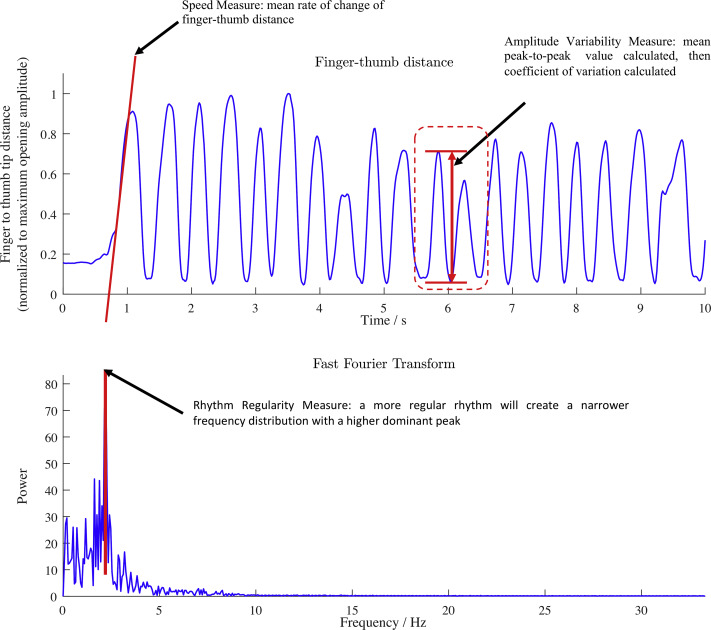
\includegraphics[width=1\textwidth]{grafica}
	\caption{Gráficas donde se visualiza la obtención de la velocidad y de la amplitud (arriba) y la obtención del ritmo (abajo)~\cite{goetz2008mds}.}
	\label{fig:grafica}
\end{figure}

Finalmente, se analizaron los datos y se obtuvieron conclusiones positivas ya que las diferencias de una persona que padece Parkinson de otra que no son notorias en este tipo de movimientos.

El experimento de este proyecto se realizó con 138 manos, tanto derecha como izquierda, de los cuales 39 tenían Parkinson y 30 no.

\subsection{A computer vision framework for finger-tapping evaluation in Parkinson's disease}
Este proyecto~\cite{khan2014computer} trata de identificar el Parkinson mediante el movimiento de la pinza, pero añadiendo además un reconocimiento facial, con el cual mejorar la obtención de los datos.

Para ello, se siguió el diagrama que se observa en la figura \ref{fig:diagramacara} con los siguientes pasos:
 
\begin{enumerate}
	\item Detectar la cara de la persona mediante un rectángulo y las dos regiones donde está cada mano. 
	\item Recoger las coordenadas del movimiento de las manos mediante el dedo índice. 
	\item Normalizar las coordenadas respecto al rectángulo que recuadra la cara de la persona. 
	\item Extraer las características de cada apertura y cierre de la pinza. 
	\item Realizar una clasificación utilizando una máquina de soporte vectorial (SVM) para clasificar los niveles de la enfermedad.
\end{enumerate}

\begin{figure}[h]
	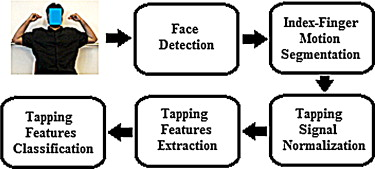
\includegraphics[width=1\textwidth]{diagrama_cara}
	\caption{Pasos que se siguieron para la realización de este proyecto~\cite{khan2014computer}.}
	\label{fig:diagramacara}
\end{figure}

El paso de la detección de la cara está basado en que el tamaño de la mano de una persona adulta es muy parecido a la altura de su cara, por lo que se puede realizar una normalización de los datos obtenidos de la mano con respecto a la cara, la cual se realiza en el tercer paso, para así tener en cuenta la distancia a la que está la cámara y que no afecte al resultado. Por otro lado, se detectan a la vez las manos para poder procesarlas en los pasos posteriores. Para esta detección, se utilizó la biblioteca OpenCV.

Para el siguiente paso, el de la detección del movimiento de los dedos, se realiza un análisis de la diferencia entre los cuatro fotogramas anteriores y los 4 posteriores para conocer el movimiento de las manos, ambas de forma separada, tal y como se aprecia en la figura \ref{fig:procesamientomanos}. Para que exista movimiento, se considera que tiene que haber una diferencia absoluta de 40 píxeles o más, ya que menos representa movimiento insignificante.

\begin{figure}[h]
	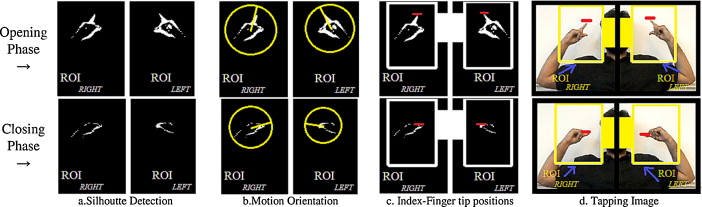
\includegraphics[width=1\textwidth]{procesamiento_manos}
	\caption{Detección de la silueta de cada mano (a), orientación del movimiento (b), posiciones del los dedos índice (c) y la imagen actual (d)~\cite{khan2014computer}.}
	\label{fig:procesamientomanos}
\end{figure}

Una vez obtenidos las coordenadas del movimiento del paso anterior, en el tercer paso, estas se calibran utilizando la cara de la persona, para normalizar los datos y que no varíen de la distancia a la cámara. Para comprobar que el algoritmo de normalización estaba ajustando correctamente los valores, se realizó una comparación del algoritmo con la utilización de marcadores de color rojo puestos en los dedos, dando el resultado que se aprecia en la figura \ref{fig:comparacioncara}. Estos marcadores de color rojo, fueron procesados con el espacio HSV, asegurándose además de que no hubiera ningún otro elemento rojo que pudiera interferir.

\begin{figure}[h]
	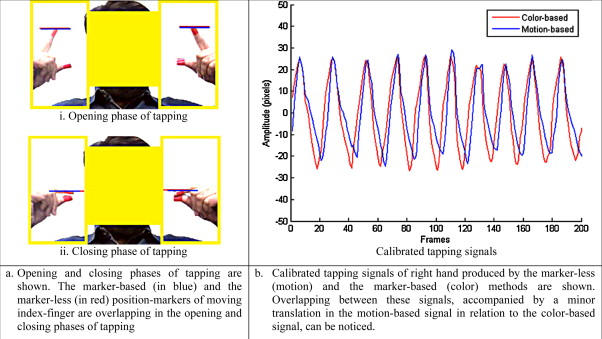
\includegraphics[width=1\textwidth]{comparacion_cara}
	\caption{Marcadores rojos puestos en los dedos para detectar la distancia (a) y comparación del algoritmo (azul) y el procesado de los marcadores (rojo) para conocer si el algoritmo ajustaba correctamente (b)~\cite{khan2014computer}.}
	\label{fig:comparacioncara}
\end{figure}

En el penúltimo paso, se extraen a partir de las coordenadas normalizadas del apartado anterior características para poder realizar una clasificación. Hubo que tener en cuenta que, generalmente, las mujeres realizan el movimiento de forma más lenta que los hombres, al igual que sucede con la mano dominante y la no dominante, pues la primera es más rápida. Las características más importantes que se extrajeron fueron: velocidad, amplitud, ritmo y comparación entre franjas horarias.

En el último paso, estas características fueron utilizadas para entrenar un clasificador, con el cual sea capaz de clasificar cada persona con el nivel de Parkinson según la escala UPDRS para el \textit{finger-tapping}, que es el tipo de movimiento que se utilizó en el proyecto. Una vez obtenidos el modelo con las predicciones, se analizaron y se concluyó que esta forma de detectar el Parkinson es viable, principalmente porque es más económico que otro tipo de detección, la cual puede necesitar de equipo costoso, y no requiere de una experiencia para poder utilizar el software.

Este experimento se realizó con los pacientes del centro clínico DIREQT (\textit{Duodopa Infusion: Randomized Efficacy and Quality of life Trial}). Había mezcla de sexos y las edades estaban comprendidas entre los 50 y 75 años. Cada grabación se realizó a lo largo del día a diferentes horas con el fin de poder obtener posibles diferencias dependiendo del momento del día, obteniendo 17 grabaciones de cada paciente.

\subsection{Tabla de medidas}
En esta sección se recoge de manera resumida en una tabla aquellas medidas que han sido utilizadas en los trabajos expuestos anteriormente y en este TFG.

\begin{table}[h]
	\begin{center}
		\begin{tabular}{| c | c | c | c | c | c |}
			\hline
			Trabajo & Amplitud & Tiempo & Velocidad & Ritmo & Comparación \\ \hline
			1 &  &  &  &  & X \\
			2 & X & X & X & X & \\ 
			3 & X & & X & X & \\
			4 & X & & X & X & X \\
			Este trabajo & X &  &  &  & \\ \hline
		\end{tabular}
		\caption{Tabla que resume las medidas utilizadas para detectar el Parkinson.}
		\label{tab:fruta}
	\end{center}
\end{table}
